\section{Building matrices from XML files}

In this file, we briefly describe how matrices are built from files.

\paragraph{Building blocks}
\reffigt{fig:blocks} shows the blocks that are used to build the final matrices.
\begin{figure}
  \centering
  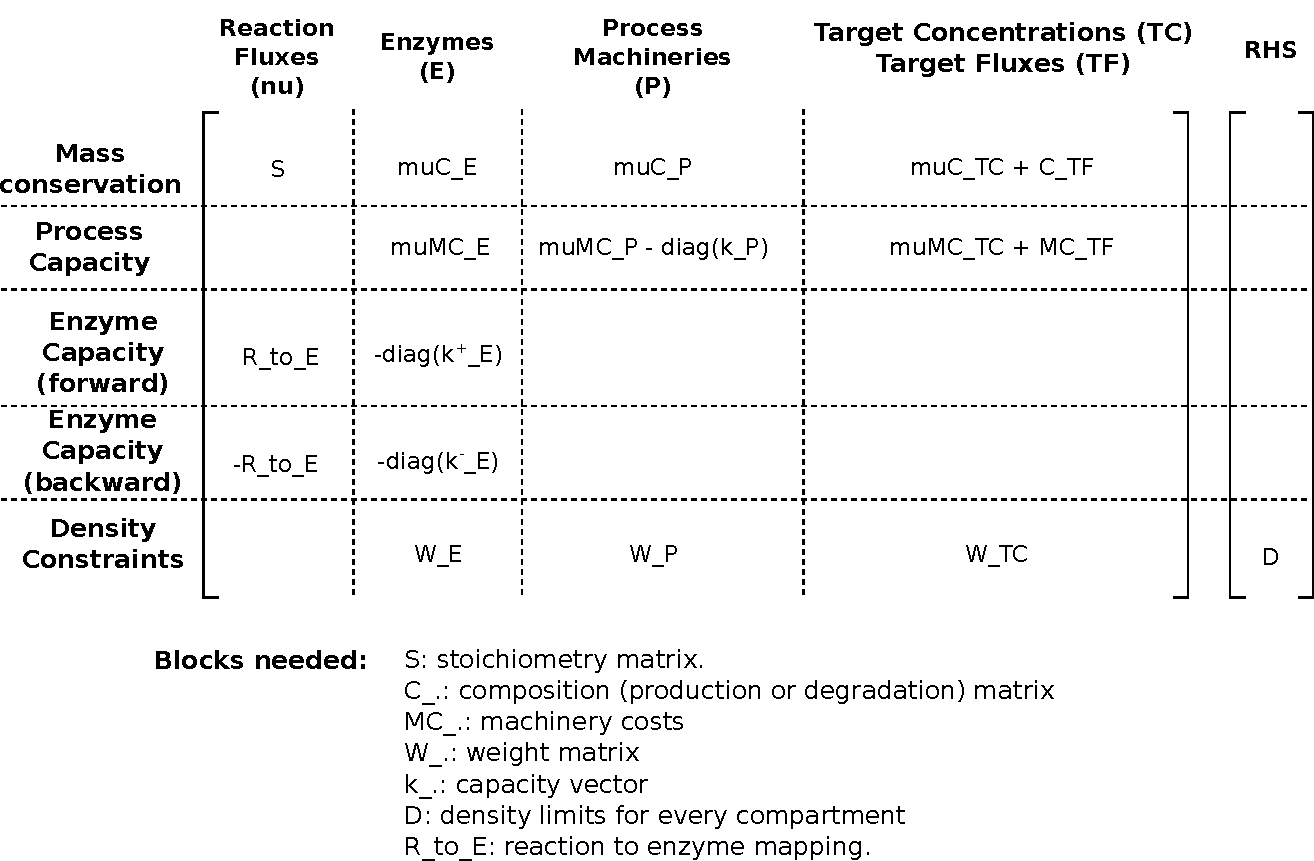
\includegraphics[width=\linewidth]{blocks}
  \caption{Blocks that need to be assembled.
  There is also a vector of constraint signs that is omitted here
  (E for equality, L for lower than, G for greater than).}
  \label{fig:blocks}
\end{figure}

\paragraph{Stoichiometry matrix}
The stoichiometry matrix is built from metabolic reactions.
External metabolites are removed from the metabolite pool.

\paragraph{Density limits}
Density limits are simply extracted from RBADensity and assembled into a vector (one coefficient per compartment).

\paragraph{Species matrices}
\reffigt{fig:species_matrices} shows how macromolecules are broken down
into matrices describing their composition, machinery cost and weight.
In the end, they are merged into a single matrix describing composition,
machinery cost and weight of all metabolites and macromolecules.
\begin{figure}
  \centering
  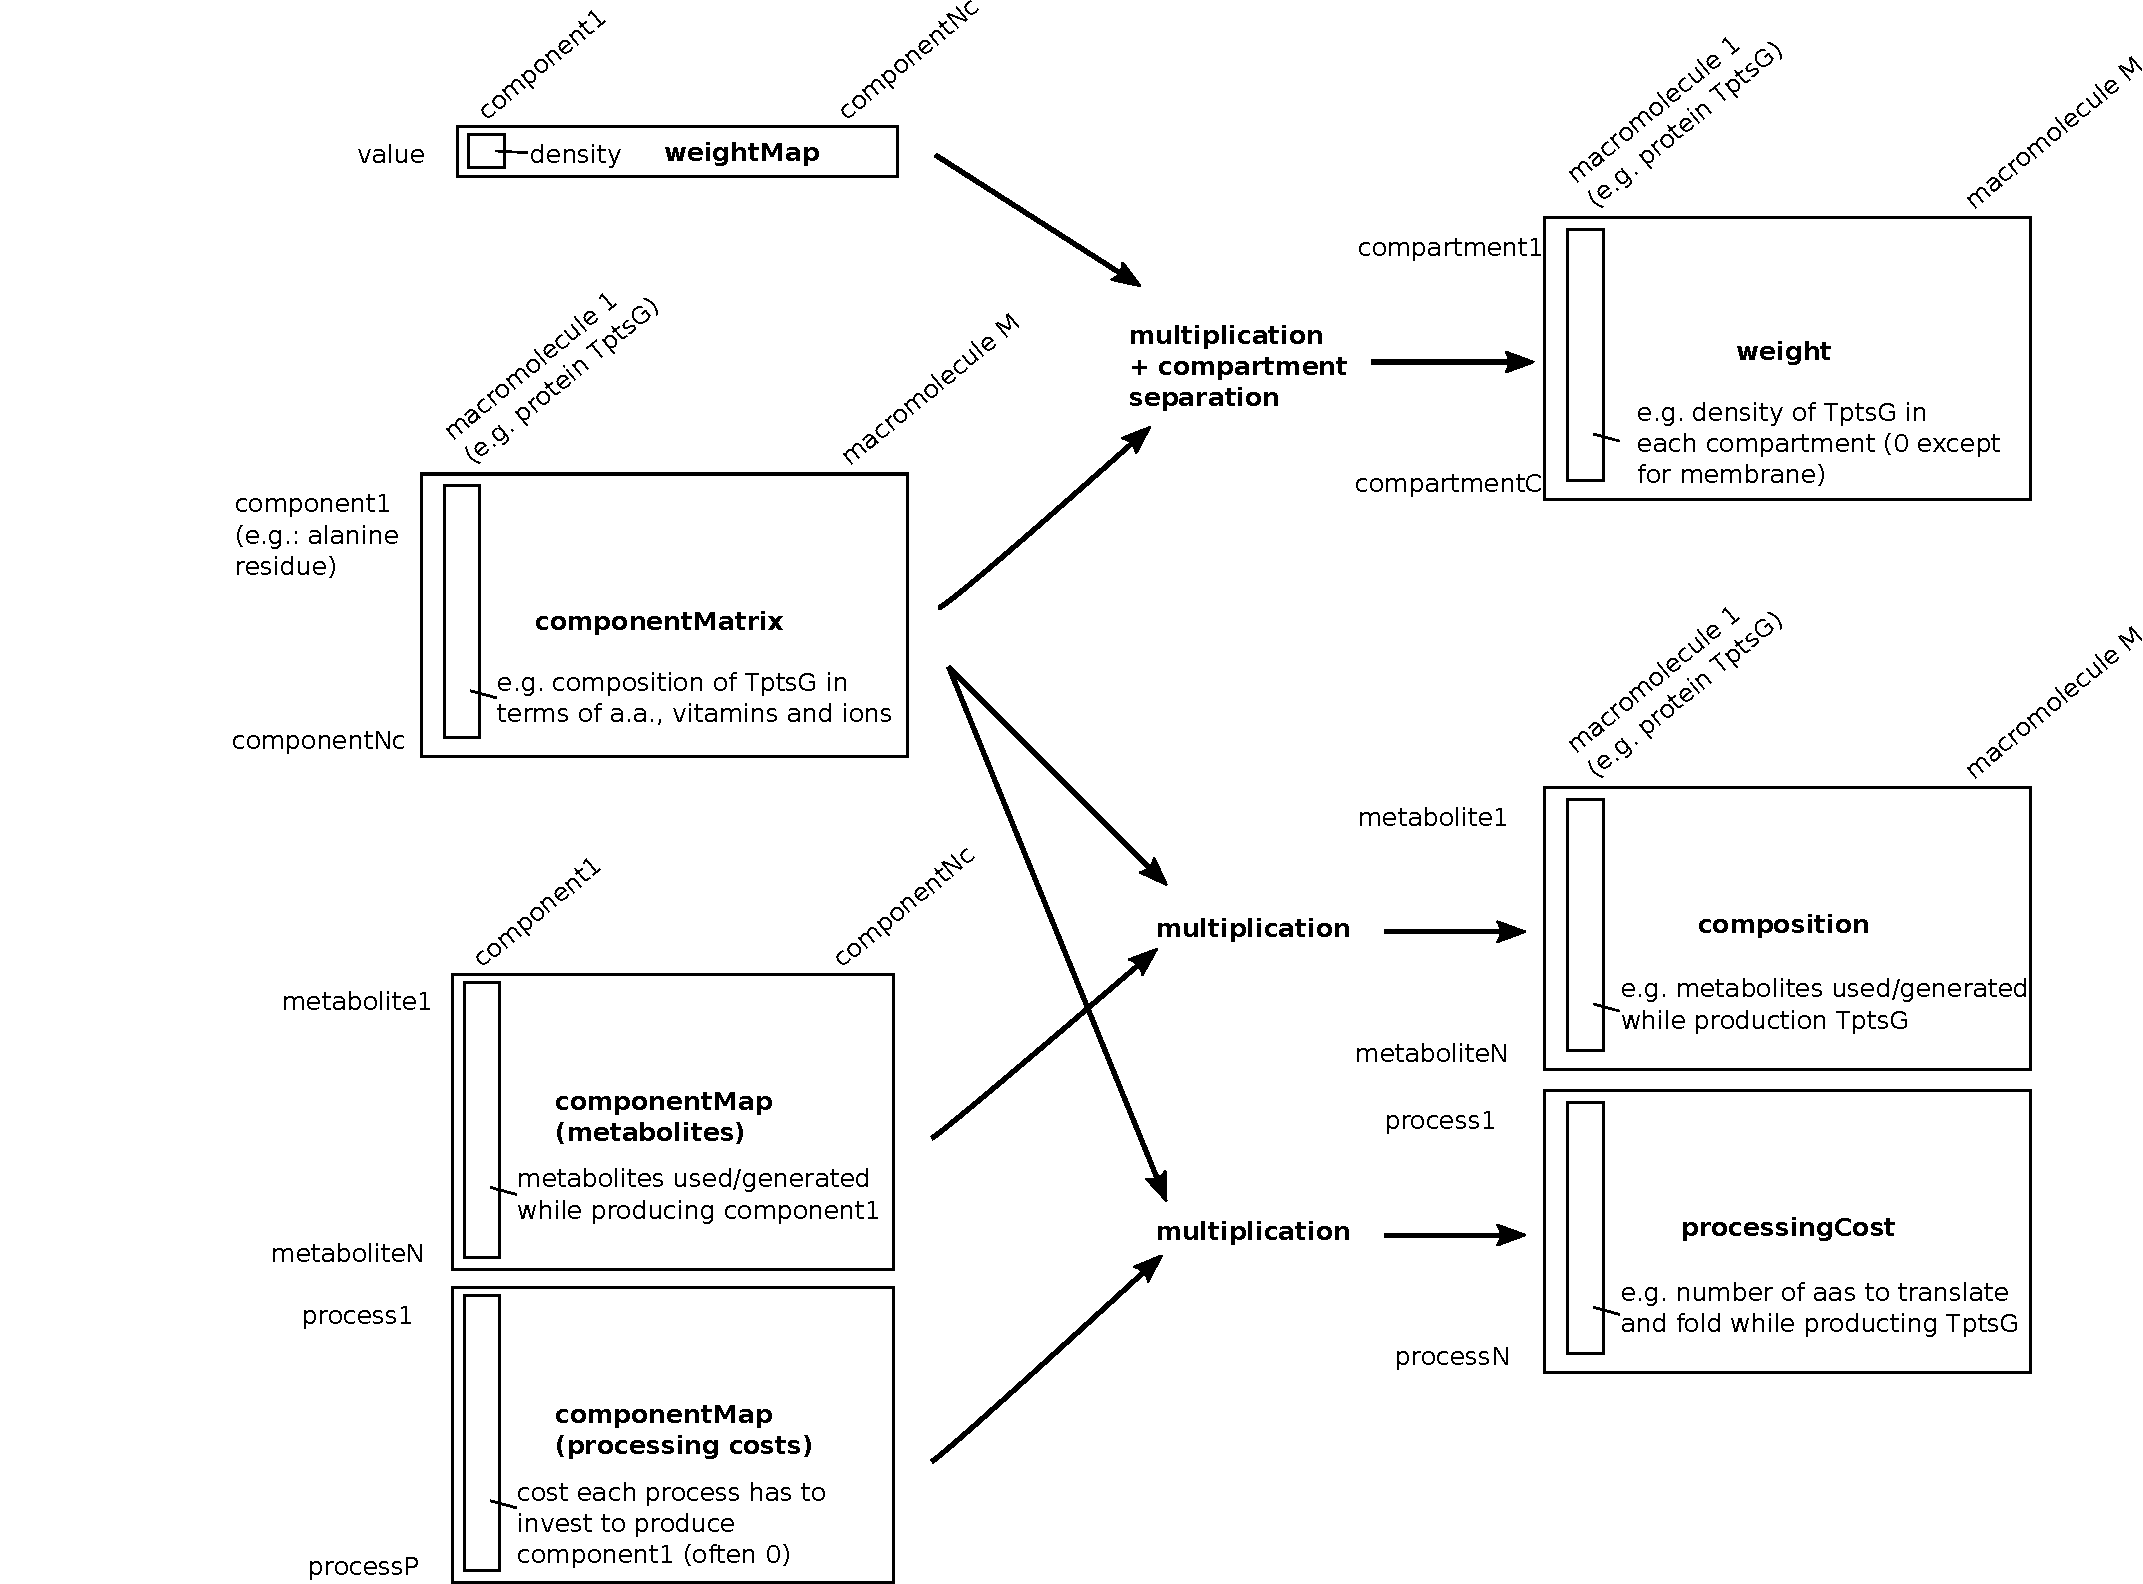
\includegraphics[width=\linewidth]{species_matrices}
  \caption{Matrices extracted from macromolecule information.
  An example is given with proteins but in the end,
  they contain all macromolecules and all internal metabolites.}
  \label{fig:species_matrices}
\end{figure}

\paragraph{Enzyme and machinery matrices}
\reffigt{fig:machinery_matrices} shows how enzyme and process machinery matrices are built.
\begin{figure}
  \centering
  \includegraphics[width=\linewidth]{machinery_matrices}
  \caption{Every machinery can be described by a reaction matrix.
  Reactants are species (metabolites or macromolecules) needed to build the machinery
  and products are byproducts of the assembly process.
  Through matrix multiplication with the species matrices,
  we can deduce its composition, weight and machinery cost.}
  \label{fig:machinery_matrices}
\end{figure}

\paragraph{Target matrices}
Targets are either metabolites or macromolecules.
Their composition, machinery cost and weight can be extracted as columns from the species matrices.
